\documentclass[12pt,a4paper]{article}

% ─── 1. PACKAGES ──────────────────────────────────────────────────────────────
\usepackage[utf8]{inputenc}
\usepackage[T1]{fontenc}
\usepackage{amsmath, amssymb}
\usepackage{geometry}
\usepackage{graphicx}
\usepackage{xcolor}
\usepackage{listings}
\usepackage{hyperref}
\usepackage{booktabs}
\usepackage{enumitem}
\usepackage{tcolorbox}
\usepackage{mdframed}
\usepackage{fancyhdr}
\usepackage{titlesec}
\usepackage{tikz} % Untuk menggambar diagram state Automata
\usetikzlibrary{automata, positioning, arrows.meta}

% Font Settings
\usepackage{newtxtext,newtxmath} % Times New Roman
\usepackage{courier}             % Courier New untuk kode

\geometry{margin=2.5cm}

% ─── 2. WARNA TEMA ────────────────────────────────────────────────────────────
\definecolor{codebg}{RGB}{245,247,250}
\definecolor{codeframe}{RGB}{180,195,215}
\definecolor{keywordcolor}{RGB}{0,112,192}
\definecolor{commentcolor}{RGB}{100,160,100}
\definecolor{stringcolor}{RGB}{180,70,50}
\definecolor{notebg}{RGB}{255,249,230}
\definecolor{noteframe}{RGB}{230,180,50}
\definecolor{tipbg}{RGB}{230,245,235}
\definecolor{tipframe}{RGB}{50,160,90}
\definecolor{sectioncolor}{RGB}{30,80,150}

% ─── 3. STYLE SECTION & TOC ───────────────────────────────────────────────────
\titleformat{\section}{\Large\bfseries\color{sectioncolor}}{}{0em}{\thesection\quad}[\titlerule]
\titleformat{\subsection}{\large\bfseries\color{sectioncolor!80}}{}{0em}{\thesubsection\quad}

% Style Table of Contents
\usepackage{tocloft}
\renewcommand{\cftsecleader}{\cftdotfill{\cftdotsep}}
\renewcommand{\cftsecfont}{\bfseries\color{sectioncolor}}

% ─── 4. LISTINGS (CODE STYLE) ─────────────────────────────────────────────────
\lstdefinestyle{customstyle}{
  basicstyle=\ttfamily\small,
  backgroundcolor=\color{codebg},
  frame=single,
  rulecolor=\color{codeframe},
  keywordstyle=\bfseries\color{keywordcolor},
  commentstyle=\itshape\color{commentcolor},
  stringstyle=\color{stringcolor},
  numbers=left,
  numberstyle=\tiny\color{gray},
  breaklines=true,
  tabsize=4,
  showstringspaces=false
}
\lstset{style=customstyle}

% ─── 5. KOTAK CATATAN (MD-FRAME) ──────────────────────────────────────────────
\newmdenv[
  backgroundcolor=notebg, linecolor=noteframe, linewidth=2pt,
  leftline=true, topline=false, rightline=false, bottomline=false,
  innerleftmargin=10pt, innertopmargin=6pt, innerbottommargin=6pt, skipabove=8pt
]{notebox}

\newmdenv[
  backgroundcolor=tipbg, linecolor=tipframe, linewidth=2pt,
  leftline=true, topline=false, rightline=false, bottomline=false,
  innerleftmargin=10pt, innertopmargin=6pt, innerbottommargin=6pt, skipabove=8pt
]{tipbox}

% ─── 6. HEADER & FOOTER ───────────────────────────────────────────────────────
\pagestyle{fancy}
\fancyhf{}
\fancyhead[L]{\small\textit{Teori Bahasa dan Automata}}
\fancyhead[R]{\small\textit{Modul Pembelajaran -- $\epsilon$-NFA}}
\fancyfoot[C]{\thepage}
\renewcommand{\headrulewidth}{0.4pt}

% ─── 7. DATA COVER ────────────────────────────────────────────────────────────
\title{
  {\LARGE\bfseries TEORI BAHASA DAN AUTOMATA}\\[0.5em]
  {\large Modul Pembelajaran: Epsilon NFA ($\epsilon$-NFA)}\\[0.8em]
  {\normalsize Penjelasan mendalam mengenai transisi gaib (epsilon), cara menghitung epsilon-closure, dan trik merancang mesin automata yang fleksibel dengan banyak studi kasus.}
}
\author{}
\date{}

% ==============================================================================
\begin{document}

\maketitle
\thispagestyle{fancy}
\tableofcontents
\newpage

% ─── KONTEN MATERI ─────────────────────────────────────────────────────────────

\section{Mengenal Epsilon NFA ($\epsilon$-NFA)}

\subsection{Apa Itu Transisi Epsilon?}
Kalau di materi NFA biasa kita udah tahu kalau mesin bisa bercabang atau punya jalan buntu, sekarang kita kenalan sama kekuatan utamanya: \textbf{Transisi Epsilon ($\epsilon$)}. Di beberapa literatur, simbol ini kadang ditulis pakai lambda ($\lambda$).

Bayangin transisi epsilon ini kayak \textbf{jalan pintas atau pintu teleportasi}. Biasanya, buat pindah dari satu \textit{state} ke \textit{state} lain, mesin butuh "bayaran" berupa ngebaca satu karakter dari pita input. Nah, dengan panah $\epsilon$, mesin diizinkan pindah ke state tujuan \textbf{secara gratis}, tanpa perlu ngebaca, menggeser, atau mengonsumsi huruf apa pun dari pita!

\begin{notebox}
\textbf{Analogi Epsilon ($\epsilon$)} \\
Anggap kamu lagi main \textit{board game}. Biasanya buat maju 1 langkah, kamu harus lempar dadu dulu. Transisi $\epsilon$ ini ibarat kartu "Bebas Melangkah". Begitu kamu dapet jalan yang ada $\epsilon$-nya, kamu bisa langsung loncat ke petak berikutnya tanpa perlu nunggu giliran lempar dadu.
\end{notebox}

\subsection{Kenapa Kita Butuh $\epsilon$-NFA?}
Mungkin kamu mikir, "NFA biasa aja udah cukup kok, ngapain nambahin teleportasi segala?". Alasan terbesarnya adalah \textbf{Modularitas}.

Bikin mesin DFA atau NFA biasa untuk mendeteksi bahasa yang super panjang dan ribet itu pusing banget. Dengan $\epsilon$-NFA, kita bisa bikin mesin-mesin kecil yang tugasnya sederhana, lalu kita jahit (sambungin) mesin-mesin kecil itu pakai jalan tol $\epsilon$. Konsep ini sangat berguna pas kita belajar tentang \textit{Regular Expression} (Regex), karena setiap pola Regex pada dasarnya dibangun dari potongan-potongan $\epsilon$-NFA yang digabungin.

\newpage
\section{Definisi Formal dan $\epsilon$-Closure}

\subsection{Tupel Matematis $\epsilon$-NFA}
Secara matematika, $\epsilon$-NFA tetep pakai 5-tupel yang sama kayak NFA biasa: $M = (Q, \Sigma, \delta, q_0, F)$. Bedanya cuma ada di satu tempat, yaitu di **Fungsi Transisinya ($\delta$)**.

Pemetaan fungsi transisinya ditulis:
\[ \delta : Q \times (\Sigma \cup \{\epsilon\}) \rightarrow \mathcal{P}(Q) \]

Artinya: Sebuah \textit{state} kalau dapet input dari alfabet ($\Sigma$) \textbf{ATAU} dapet input kosong ($\epsilon$), dia bakal menghasilkan himpunan \textit{state} tujuan ($\mathcal{P}(Q)$).

\subsection{Kunci Utama: $\epsilon$-Closure}
Ini adalah konsep paling penting kalau kamu mau ngerjain soal atau merancang $\epsilon$-NFA. \textbf{$\epsilon$-Closure} (dibaca: epsilon-klosur) dari sebuah \textit{state} adalah kumpulan semua \textit{state} yang bisa didatengin dari state tersebut \textbf{hanya dengan menggunakan transisi $\epsilon$}.

Aturan main $\epsilon$-Closure:
\begin{enumerate}
    \item Sebuah state \textbf{selalu} bisa mendatangi dirinya sendiri dengan biaya nol. Jadi, nama state itu pasti masuk ke dalam himpunan $\epsilon$-Closure-nya sendiri.
    \item Kalau dari state A ada jalan $\epsilon$ ke B, dan dari B ada jalan $\epsilon$ ke C, maka $\epsilon$-Closure dari A meliputi A, B, dan C. Sifatnya menjalar kayak air tumpah!
\end{enumerate}

\begin{figure}[h]
    \centering
    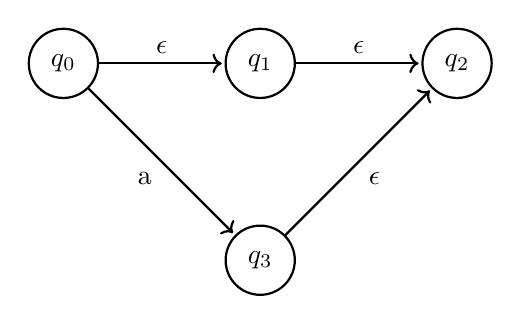
\begin{tikzpicture}[shorten >=1pt,node distance=2.5cm,on grid,auto, thick]
       \node[state] (q0) {$q_0$};
       \node[state] (q1) [right=of q0] {$q_1$};
       \node[state] (q2) [right=of q1] {$q_2$};
       \node[state] (q3) [below=of q1] {$q_3$};

       \path[->] 
       (q0) edge node {$\epsilon$} (q1)
            edge node [swap] {a} (q3)
       (q1) edge node {$\epsilon$} (q2)
       (q3) edge node [swap] {$\epsilon$} (q2);
    \end{tikzpicture}
    \caption{Contoh Sederhana untuk Menghitung $\epsilon$-Closure}
\end{figure}

Mari kita hitung $\epsilon$-Closure dari diagram di atas:
\begin{itemize}
    \item $\epsilon\text{-Cl}(q_0) = \{q_0, q_1, q_2\}$ (Bisa ke dirinya sendiri, loncat ke $q_1$, dan karena $q_1$ nyambung ke $q_2$, dia ikut tembus ke $q_2$).
    \item $\epsilon\text{-Cl}(q_1) = \{q_1, q_2\}$
    \item $\epsilon\text{-Cl}(q_2) = \{q_2\}$ (Nggak ada panah $\epsilon$ yang keluar dari dia).
    \item $\epsilon\text{-Cl}(q_3) = \{q_3, q_2\}$
\end{itemize}

\newpage
\section{Kumpulan Studi Kasus Perancangan $\epsilon$-NFA}

Di bagian ini kita bakal lihat betapa fleksibelnya $\epsilon$-NFA buat nyelesaiin masalah-masalah yang rumit kalau dikerjain pakai DFA.

\subsection{Kasus 1: Pilihan Paralel (Kondisi ATAU)}
Kita mau bikin mesin buat mendeteksi string yang memuat "11" berurutan \textbf{ATAU} "00" berurutan. Ini kasus klasik di mana $\epsilon$-transition sangat bersinar.

\begin{figure}[h]
    \centering
    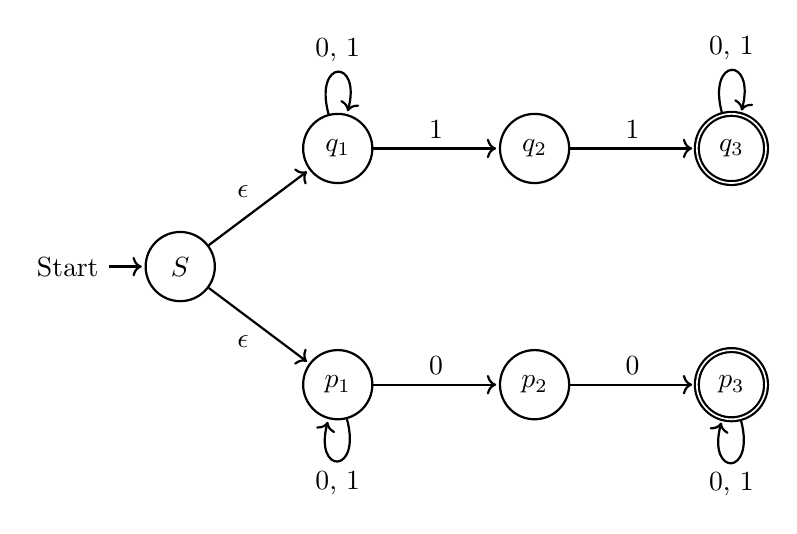
\begin{tikzpicture}[shorten >=1pt,node distance=2.5cm,on grid,auto, thick]
       \node[state,initial,initial text=Start] (S) {$S$};
       
       % Cabang 11
       \node[state] (q1) [above right=1.5cm and 2cm of S] {$q_1$};
       \node[state] (q2) [right=of q1] {$q_2$};
       \node[state,accepting] (q3) [right=of q2] {$q_3$};

       % Cabang 00
       \node[state] (p1) [below right=1.5cm and 2cm of S] {$p_1$};
       \node[state] (p2) [right=of p1] {$p_2$};
       \node[state,accepting] (p3) [right=of p2] {$p_3$};

       \path[->] 
       (S) edge node [above left] {$\epsilon$} (q1)
           edge node [below left] {$\epsilon$} (p1)
           
       (q1) edge [loop above] node {0, 1} (q1)
            edge node {1} (q2)
       (q2) edge node {1} (q3)
       (q3) edge [loop above] node {0, 1} (q3)
       
       (p1) edge [loop below] node {0, 1} (p1)
            edge node {0} (p2)
       (p2) edge node {0} (p3)
       (p3) edge [loop below] node {0, 1} (p3);
    \end{tikzpicture}
    \caption{Cabang Paralel menggunakan $\epsilon$-NFA}
\end{figure}

Begitu mesin nyala, kloningannya langsung pecah dua secara otomatis. Satu tim di atas fokus mantau pola "11", satu tim di bawah fokus mantau pola "00". Kalau salah satu tim berhasil nyampe \textit{Final State}, string langsung diterima. Nggak perlu repot bikin panah silang antar \textit{state}.

\subsection{Kasus 2: Elemen Opsional (Boleh Ada, Boleh Nggak)}
Misalkan kita mau mendeteksi penulisan angka desimal yang boleh pakai tanda plus (+), minus (-), atau \textbf{nggak pakai tanda sama sekali}. Alfabetnya $\Sigma = \{+, -, d\}$ (anggap aja 'd' itu singkatan dari digit angka apa pun).

\begin{figure}[h]
    \centering
    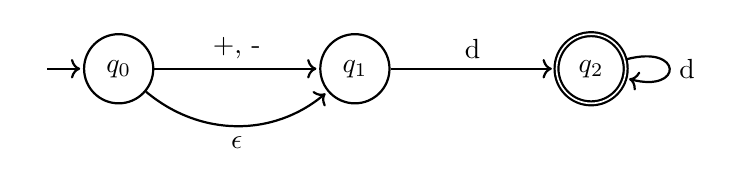
\begin{tikzpicture}[shorten >=1pt,node distance=3cm,on grid,auto, thick]
       \node[state,initial,initial text=] (q0) {$q_0$};
       \node[state] (q1) [right=of q0] {$q_1$};
       \node[state,accepting] (q2) [right=of q1] {$q_2$};

       \path[->] 
       (q0) edge node {+, -} (q1)
            edge [bend right=40] node [swap] {$\epsilon$} (q1)
       (q1) edge node {d} (q2)
       (q2) edge [loop right] node {d} (q2);
    \end{tikzpicture}
    \caption{Transisi $\epsilon$ untuk \textit{Bypassing} (Melewati) State}
\end{figure}

Di sini, panah $\epsilon$ berfungsi sebagai jalan \textit{bypass}.
\begin{itemize}
    \item Kalau inputnya "+d" atau "-d", mesin bakal milih jalur normal baca simbol tanda, lalu masuk ke $q_1$, lalu baca 'd' dan diterima di $q_2$.
    \item Kalau inputnya cuma "d" (tanpa tanda), mesin tinggal pilih jalan tol $\epsilon$ buat langsung lompat ke $q_1$ tanpa baca apa-apa, lalu baca 'd' dan tetep diterima dengan sukses!
\end{itemize}

\subsection{Kasus 3: Perulangan Penuh (Kleene Star)}
Kasus ini paling sering nongol di Regex. Kita mau nerima bahasa $a^*b^*c^*$. Artinya: huruf 'a' dulu (boleh nggak ada), lanjut huruf 'b' (boleh nggak ada), ditutup huruf 'c' (boleh nggak ada).

\begin{figure}[h]
    \centering
    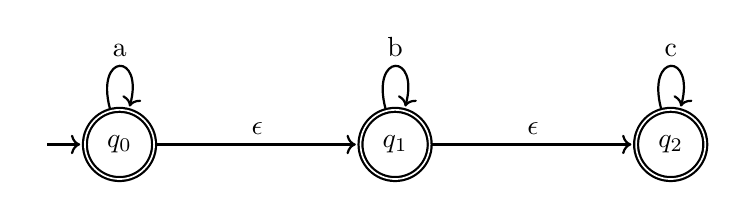
\begin{tikzpicture}[shorten >=1pt,node distance=3.5cm,on grid,auto, thick]
       \node[state,initial,initial text=,accepting] (q0) {$q_0$};
       \node[state,accepting] (q1) [right=of q0] {$q_1$};
       \node[state,accepting] (q2) [right=of q1] {$q_2$};

       \path[->] 
       (q0) edge [loop above] node {a} (q0)
            edge node {$\epsilon$} (q1)
       (q1) edge [loop above] node {b} (q1)
            edge node {$\epsilon$} (q2)
       (q2) edge [loop above] node {c} (q2);
    \end{tikzpicture}
    \caption{Penggunaan $\epsilon$-NFA untuk Perulangan Bersambung}
\end{figure}

Karena semua \textit{state} adalah \textit{Final State}, dan disatukan pakai panah $\epsilon$, kita bisa ngerasain fleksibilitas yang luar biasa:
\begin{itemize}
    \item Kalau kita masukin string kosong (nggak ngetik apa-apa), posisinya tetep di $q_0$ (Final) $\rightarrow$ Diterima.
    \item Kalau masukin "ac", mesin baca 'a' di $q_0$, terus seketika pindah pakai $\epsilon$ lewatin $q_1$ dan langsung ke $q_2$ buat baca 'c' $\rightarrow$ Diterima.
    \item Kalau masukin "ca", mesin bakal meluncur ke $q_2$ buat baca 'c', tapi pas mau baca 'a' dia gagal karena nggak ada panah mundur $\rightarrow$ Ditolak.
\end{itemize}

\subsection{Kasus 4: Penggabungan Dua Mesin (Concatenation)}
Anggaplah kita punya dua mesin terpisah. Mesin pertama nyari pola yang huruf terakhirnya "a". Mesin kedua nyari pola yang huruf pertamanya "b". Kita pengen gabungin mesin ini biar dia nerima kata yang ada transisi "ab" di tengahnya.

\begin{figure}[h]
    \centering
    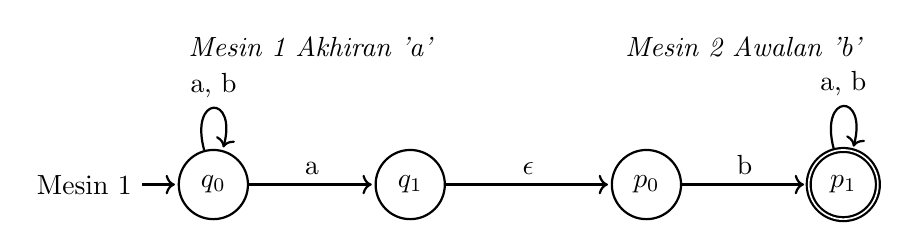
\begin{tikzpicture}[shorten >=1pt,node distance=2.5cm,on grid,auto, thick]
       \node[state,initial,initial text=Mesin 1] (q0) {$q_0$};
       \node[state] (q1) [right=of q0] {$q_1$};
       
       \node[state] (p0) [right=3cm of q1] {$p_0$};
       \node[state,accepting] (p1) [right=of p0] {$p_1$};

       \path[->] 
       (q0) edge [loop above] node {a, b} (q0)
            edge node {a} (q1)
       
       (q1) edge node [above] {$\epsilon$} (p0)
       
       (p0) edge node {b} (p1)
       (p1) edge [loop above] node {a, b} (p1);
       
       \node[above] at (1.25, 1.5) {\textit{Mesin 1 Akhiran 'a'}};
       \node[above] at (6.75, 1.5) {\textit{Mesin 2 Awalan 'b'}};
    \end{tikzpicture}
    \caption{Penggabungan Mesin menggunakan Jembatan $\epsilon$}
\end{figure}

Transisi $\epsilon$ di sini bertindak sebagai **jembatan**. Tanpa $\epsilon$, kita harus narik ulang panah-panah dengan rumus yang ribet. Pakai $\epsilon$, kita tinggal ambil \textit{Final State} dari Mesin 1 (hapus status finalnya), tarik garis $\epsilon$, tempel ke \textit{Initial State} Mesin 2. Beres!

\newpage
\section{Cara Mengeksekusi / Tracing String pada $\epsilon$-NFA}

Di bagian ini, kita bahas gimana sih cara ngebaca atau memproses string kalau ada $\epsilon$-nya? Logika jalannya mesin adalah: **Tutup dulu pakai Epsilon, baru Baca, terus Tutup lagi**.

Secara urutan komputasi:
\begin{enumerate}
    \item Hitung $\epsilon$-Closure dari \textit{state} saat ini. Ini nentuin kloningan awal kita ada di mana aja.
    \item Dari semua kloningan itu, baca 1 karakter input dan gerak sesuai panahnya.
    \item Setelah pindah, hitung LAGI $\epsilon$-Closure dari tempat-tempat baru tersebut.
\end{enumerate}

\textbf{Contoh Simulasi Tracing:}\\
Kita pakai mesin di Kasus 3 (Pola $a^*b^*c^*$) dan kita masukin string \textbf{"bc"}.
\begin{itemize}
    \item \textbf{Start:} Posisi awal di $q_0$. Jangan lupa langsung hitung $\epsilon$-Closure nya.\\
    $\epsilon\text{-Cl}(q_0) = \{q_0, q_1, q_2\}$.\\
    Artinya, sebelum baca karakter apa pun, mesin kita udah ada di 3 tempat sekaligus!
    
    \item \textbf{Baca Karakter Pertama 'b':}\\
    Kita tanya satu-satu:
    - $q_0$ baca 'b'? Gagal (jalan buntu).\\
    - $q_1$ baca 'b'? Tembus ke $q_1$.\\
    - $q_2$ baca 'b'? Gagal (jalan buntu).\\
    Hasil bacanya cuma ada di $q_1$. Langsung kita hitung penutupnya: $\epsilon\text{-Cl}(q_1) = \{q_1, q_2\}$.\\
    Posisi mesin sekarang setelah baca 'b' ada di $\{q_1, q_2\}$.

    \item \textbf{Baca Karakter Kedua 'c':}\\
    Kita tanya lagi dari posisi sekarang:
    - $q_1$ baca 'c'? Gagal (jalan buntu).\\
    - $q_2$ baca 'c'? Tembus ke $q_2$.\\
    Hasil bacanya cuma ada di $q_2$. Tutup lagi: $\epsilon\text{-Cl}(q_2) = \{q_2\}$.
\end{itemize}

String habis! Posisi akhir mesin ada di himpunan $\{q_2\}$. Karena $q_2$ adalah \textit{Final State}, maka string "bc" dinyatakan \textbf{Diterima}.

\end{document}